\documentclass[a4paper, english]{article}

\usepackage[utf8]{inputenc}
\usepackage[parfill]{parskip}
\usepackage[english]{babel}
\usepackage{listings}
\usepackage{hyperref}
\usepackage{graphicx}

\title{Automated testing in Java}
\author{Martin Pola}
\date{}

\hypersetup{
    colorlinks=true,
    linkcolor=blue,
    filecolor=blue,      
    urlcolor=blue
}

\lstset{
    basicstyle=\ttfamily,
    columns=fullflexible,
}

\begin{document}
    \maketitle

    \section{Setup IntelliJ}
        Follow the steps below to get started with automated testing in IntelliJ.

        \begin{enumerate}
            \item From Canvas, download the compressed folder \texttt{TestFramework.zip} and extract it in a safe location on your computer, e.g. on your desktop.

            \item In IntelliJ, navigate to \emph{File} -> \emph{New} -> \emph{Project from Existing Sources...} and select the extacted \emph{TestFramework} as the folder to base your project on. Go through the import guide.

            \item When the project has been created, click \emph{File} -> \emph{Project Structure...} in the menu. Under \emph{Modules}, make sure to mark the \texttt{main} folder as \emph{Sources} and the \texttt{test} folder as \emph{Tests}.

            \item Open the file \texttt{src/test/MyUnitTests.java} and look at the \emph{import} statements right above the class definition.

            \item Click on the red \emph{junit} text and choose to add JUnit4 to class path, as in the image below. \\
             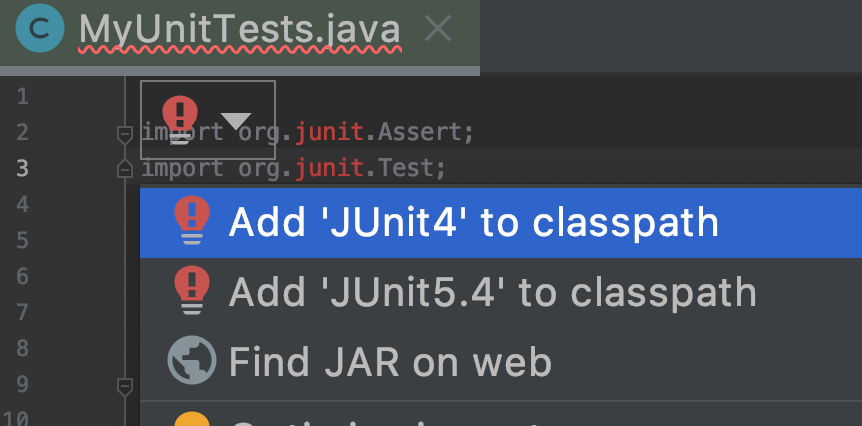
\includegraphics[width=\textwidth]{add-junit4.png}

            \item Press \emph{OK} in the dialog window that appears.
        \end{enumerate}

        If everything is correctly set up, you should now be able to run all unit tests by right-clicking on the green \texttt{test} folder in the project file tree. See the image below.

        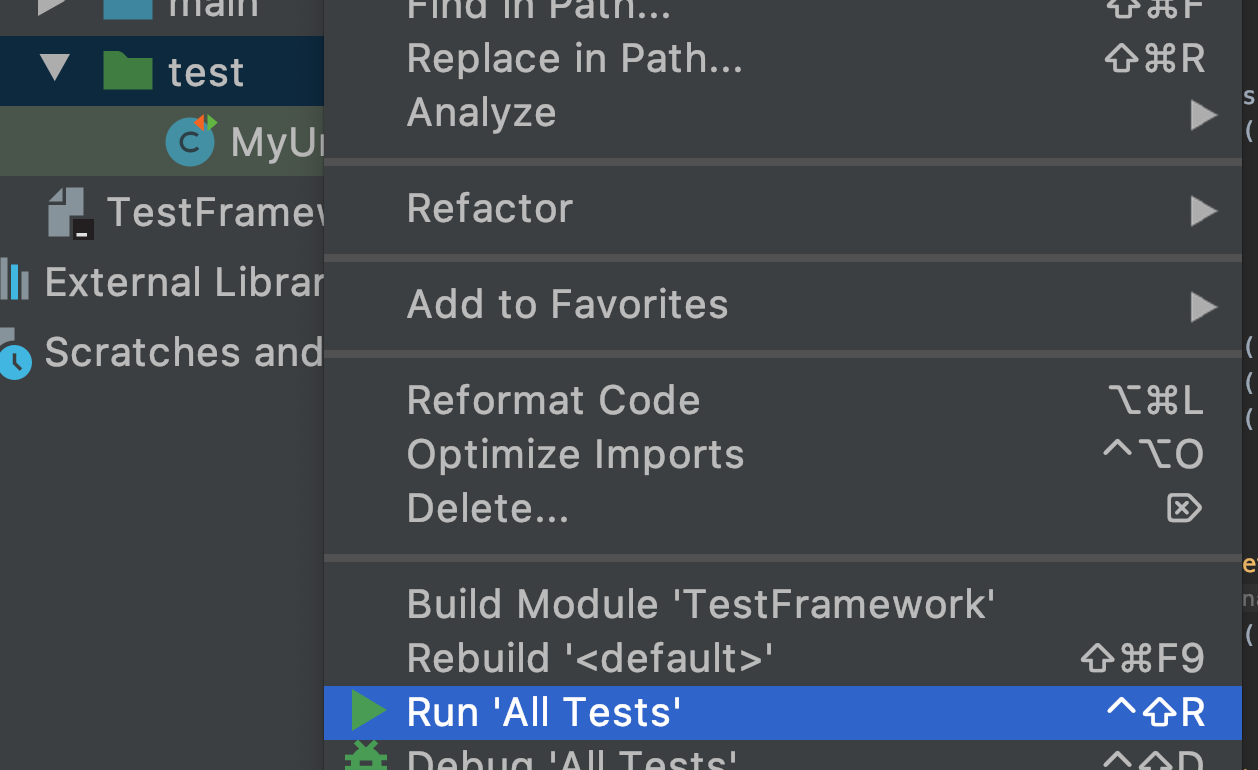
\includegraphics[width=\textwidth]{run-tests.png}

    \section{Task}
        When all tests run, they initially fail. Inspect the test cases to see what they do, and modify the files in \texttt{src/main} so that the test cases pass. Note that you are \underline{not allowed} to edit the test cases themselves -- all work should be done in the source code in the \texttt{src/main} folder.
\end{document}